%!TEX root = ../main.tex


\begin{frame}{Aprendizado de Máquina}
\begin{itemize}
	\item Algoritmos capazes de aprender padrões por meio de exemplos, baseando-se em dados previamente disponíveis
	\bigskip
	\item As técnicas de \alert{Aprendizado de Máquina} têm sido aplicadas com sucesso em um grande número de problemas reais em diversos domínios
	\bigskip
	\item Características: natureza inferencial e a boa capacidade de generalização
	\bigskip
	\item Paradigmas de aprendizado supervisionado e não-supervisionado
\end{itemize}
\end{frame}

\begin{frame}{Redes Neurais Artificiais}
  \vskip2\baselineskip
	\begin{itemize}
		\item Inspiradas na capacidade de processamento de informações do cérebro humano
		\bigskip
		\item \alert{Neurônios artificiais} são as unidades fundamentais de uma RNA
		\item \alert{Função de ativação} fornece a resposta de um neurônio para uma dada entrada
		\bigskip
		\item Neurônios artificiais são conectados entre si na forma de uma rede e distribuídos em uma ou mais camadas ocultas
		\bigskip
		\item Algoritmo \emph{Backpropagation}
		\begin{itemize}
			\footnotesize
			\item Fase \emph{forward} -- produz uma saída para uma dada entrada
			\item Fase \emph{backwards} -- calcula a diferença entre as saídas para minimizar o erro
		\end{itemize}
	\end{itemize}
\end{frame}

\begin{frame}{\emph{Deep Learning} e Redes Neurais Convolucionais}
  \vskip2\baselineskip
\begin{itemize}
	\item \emph{Deep Learning} é uma subárea específica do Aprendizado de Máquina
	\bigskip
	\item Redes Neurais Convolucionais (CNNs):
    \begin{itemize}
      \item Possuem camadas \alert{hierárquicas} e \alert{profundas}
      \item Aproveitam-se da operação matemática denominada \alert{convolução}
      \item Destacam-se pelo reconhecimento de padrões em dados de alta dimensionalidade
    \end{itemize}

    \begin{figure}
    	\caption{Papel das camadas convolucionais e \emph{feature maps} das CNNs}
    	\label{fig:camadas-convolucionais}
    	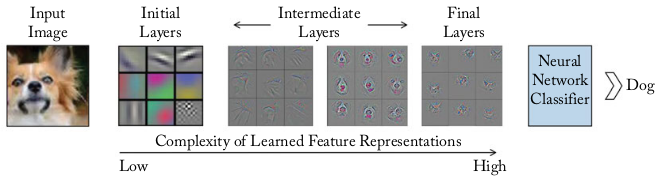
\includegraphics[width=0.5\textwidth]{./img/camadas-convolucionais}
    \end{figure}

\end{itemize}
\end{frame}


\begin{frame}{\Large{Arquiteturas Canônicas de Redes Neurais Convolucionais}}
\begin{itemize}
	\item Arquiteturas com bom desempenho em competições de \alert{Visão Computacional}
	\item Comuns ainda hoje no cenário de \emph{Deep Learning}
	\bigskip
	\item LeNet (1998)
	\item AlexNet (2012)
	\item VGG (2014)
	\item Inception (2014)
	\item ResNet (2015)
\end{itemize}

\end{frame}
